%%%--------------------------------%%%
%%% Domain
%%%--------------------------------%%%

\section{Architecture}
\label{sec:DomainC}

In this chapter the used architectural patterns, technologies, frameworks and libraries are briefly explained. First, an overall composition is given whose individual layers will then be explicitly described.


\subsection{Overall composition}
\label{sec:DomainCa}
Based on the Model-View-Controller (\ac{MVC}) architectural pattern the application is split into three major parts: the frontend, backend and persistence layer. As seen in figure \ref*{fig:overallcomposition} the frontend is in charge of the view and the backend of the model and controller.

In terms of the \ac{MVC} pattern, the view / frontend is a presentational layer accessible by the user – traditionally a user interface. The model is equivalent to the data of an application which can be persisted with any appropriate technology (e.g. a database). The data itself can be accessed, updated or deleted by the controller. Furthermore, the controller is in charge of the logic of the application \cite[p. 7]{steyerWebanwendungenMitASP2017}.

\begin{figure}[h]
	\centering
	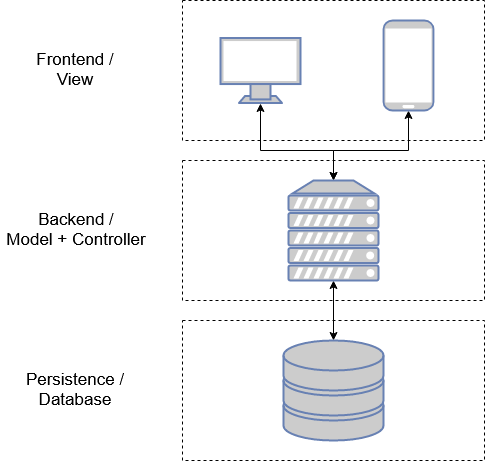
\includegraphics[width=0.6\textwidth]{Content/Domain/OverallComposition.png}
	\caption{Overall Composition}
	\cite{own representation}
	\label{fig:overallcomposition}
\end{figure}

\subsection{Frontend / View}
\label{sec:DomainCb}

The view of the application is primarly developed with React (Version 16.8.5) and Redux (Version 6.0.1).

React is a JavaScript library written by Facebook Inc. for user interface (typically web apps) developing. The major benefits from using React are components and their states. Components (e.g. an alert) are written in \ac{JSX} (a combination of JavaScript and XML) and reusable which means when written once they can be reused anywhere else in the user interface, thus duplicate source code can be avoided. In React a component can hold its own state (e.g. the alert message or alert duration) which can be used for the user interface. If the state of a component changes and is involved in the user interface React automatically updates the user interface with the new state, making the development of the user interface easier as elements do not have to be addressed manually and then adjusted with the new content \cite[p. 7-8]{stefanovDurchstartenMitReact2017}.

Even though components can pass their states in hierarchical order, having a central store for the state of the components has several benefits as simplifying the overall project structure and easier testing. Redux is a JavaScript library providing such a store and introducing further terms described in the following list:

\begin{itemize}
	\item \textbf{Action}: An action typically leads to changes in the store but does not directly adjusts it. In fact, an action is responsible for fetching data from any resource (e.g. via the controller of the backend). The collected data will then be passed to a corresponding reducer.
	\item \textbf{Reducer}: A reducer contains the business logic about how exactly the data from the action should be saved to the store (e.g. filtering the action for only necessary information).
	\item \textbf{Store}: The store contains the state of the application and can be accessed by React components \cite[p. 531-534]{freemanProReact162019}. 
\end{itemize}

Figure \ref{fig:reduxpattern} visually explains the Redux pattern.

\begin{figure}[h]
	\centering
	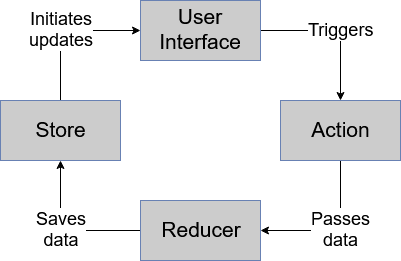
\includegraphics[width=0.6\textwidth]{Content/Domain/ReduxPattern.png}
	\caption{Redux Pattern}
	\cite{own representation}
	\label{fig:reduxpattern}
\end{figure}

\subsection{Backend}
\label{sec:DomainCc}
spring, spring boot...

\subsection{Database}
\label{sec:DomainCd}
db...

